\documentclass[11pt, a4paper, twocolumn]{article}

% Fonts and math (Elsevier-like Times style)
\usepackage{graphicx} % Required for inserting images
\usepackage{array} % For extra column formatting
\usepackage{amsmath, amssymb, cancel, siunitx, mathtools, physics2, upgreek} % for equation environment
\usepackage{float,geometry,subcaption, longtable}
\geometry{margin=2cm}
\usepackage[skip=10pt]{parskip}
\usepackage{setspace}
\usepackage{hyperref, cleveref}
\usepackage{cite, bookmark}
\usepackage{url}
\usepackage[table,xcdraw]{xcolor}
\usepackage[export]{adjustbox}
\usepackage{listings,pdfpages}
\usepackage{dblfloatfix}

% --- Abstract styling (elsarticle look)
\usepackage{abstract}
\renewcommand{\abstractnamefont}{\normalfont\bfseries}
\renewcommand{\abstracttextfont}{\normalfont}
\renewenvironment{abstract}{%
  \par\noindent\rule{\linewidth}{0.4pt}\par
  \begin{center}\bfseries Abstract\end{center}%
}{%
  \par\rule{\linewidth}{0.4pt}\par
}

% --- Section styling (similar to elsarticle
\usepackage{titlesec}
\titleformat{\section}{\normalfont\large\bfseries}{\thesection.}{0.5em}{}
\titleformat{\subsection}{\normalfont\normalsize\bfseries}{\thesubsection.}{0.5em}{}

% Table of contents styling
\usepackage{tocloft}
\cftsetindents{section}{0em}{2em}
\cftsetindents{subsection}{1em}{2em}
\renewcommand\cfttoctitlefont{\hfill\Large\bfseries}
\renewcommand\cftaftertoctitle{\hfill\mbox{}}
\renewcommand\cftfigfont{\footnotesize}
\renewcommand\cftfigpagefont{\footnotesize}
\renewcommand\cftloftitlefont{\large}

\graphicspath{ {./images/} }

\definecolor{blurple}{HTML}{5865F2}
\definecolor{backcolour}{HTML}{272823}

\hypersetup{
    colorlinks=true,
    linkcolor=black,
    urlcolor=black,
    citecolor=blurple,
}

\urlstyle{same}

\DeclareMathOperator{\sinc}{sinc}

\renewcommand{\arraystretch}{1.4}

% Python code export
\lstset{
    language=Python,
    basicstyle=\ttfamily\scriptsize,
    keywordstyle=\color{magenta},       
    commentstyle=\color{gray},        
    stringstyle=\color{teal},  
    showstringspaces=false,
    frame=single,
    breaklines=true,
    numbers=left,
    numberstyle=\tiny\color{gray}
}

\setcounter{secnumdepth}{5}
\setcounter{tocdepth}{5}

\hbadness=99999

%%%%%%%%%%%%%%%%%%%%%%%%%%%%%%%%%%%

\title{%


\includegraphics[width=0.2\linewidth]{ucd_brandmark_black.jpg} \vspace{0.5cm}\\

{\Large\bfseries UCD School of Physics}\vspace{1.5cm}\\

{\large PHYC30170 Physics Astronomy and Space Lab I}\\
{\bfseries Ramsauer-Townsend}

}
\author{Joana C.C. Adao \\ \small Student No.: 23311051}
\date{\today}

\begin{document}

% Title page - single column
\onecolumn
\maketitle

% Abstract - single column
\pagenumbering{roman}
\setcounter{page}{1}
\begin{abstract}

This experiment sought to investigate and verify the quantum phenomenon of the Ramsauer-Townsend effect for low-energy electrons incident on a noble gas, such as xenon. Using a 2D21 thyratron tube filled with xenon gas, the plate ($V_p$) and shield ($V_s$) voltages were found with multimeters across an accelerating voltage range of 0-12 V and used to calculate the respective plate ($I_p$) and shield ($I_s$) currents. To establish a scattering baseline, the xenon was frozen using liquid nitrogen to create a vacuum-like environment, for which the plate ($I_p^*$) and shield ($I_s^*$) currents were also calculated. Experimental corrections for the mean emission ($\bar{V}$) and contact ($V_c$) potentials were determined through reverse polarity measurements of the frozen xenon, yielding $\bar{V}=0.11\pm 0.045 \; \text{V}$ and $V_c = 0.0155 \pm 0.0285\; \text{V}$. While $\bar{V}$ aligned well with theoretical expectations of $\bar{V} = 0.15 \pm 0.03 \;\text{V}$, the $V_c$ value deviated significantly from the expected $V_c = 0.2 \pm 0.04 \;\text{V}$, primarily due to subjective identification of the "knee" in the saturated and retarding data groups. Despite systematic errors, the corrected scattering probability exhibited a distinct minimum of $P_{s,\text{min}}=0.0004 \pm 0.0447$ at an electron momentum of $\sqrt{V}_{\text{min}}=0.6829 \pm 0.0390\; \text{V}^{1/2}$. This contradicted the classical model of hard spherical atoms with constant scattering cross-sections and thus verified the quantum-mechanical potential well model and the wave-particle duality of electrons.

\end{abstract}

\newpage

% Table of Contents - single column
\tableofcontents

\newpage

%%%%%%%%%%%%%%%%%%%%%%%%%%%%%%%%%%%

% Start main content in two columns
\twocolumn
\pagenumbering{arabic}
\setcounter{page}{1}

\section{Introduction} \label{sec:1}

The Ramsauer-Townsend effect is a quantum mechanical phenomenon in which the scattering of low-energy electrons off noble gases, such as xenon (Xe), is observed. If this were to be described classically as hard spheres, then the scattering cross-section of the atom is expected as a constant with respect to its geometric radius and independent of the electron energy. However, the Ramsauer-Townsend effect demonstrates a sharp minimum in the cross-section at low energies around 1 eV, suggesting that the gas becomes effectively transparent to the incident electrons. \cite{kukolich1968demonstration,zwiebach2016lecture17}

\subsection{Quantum Potential Well Model}

\subsubsection{1D Model}

An electron possesses a wave-particle duality that is associated to the deBroglie wavelength $\lambda = h/p$, which determines the electron's interactions with atomic potentials with wave-like properties. \cite{young1996university}

When treated as a one-dimensional finite potential well with depth $V_0$ and width $2a$, the electron's kinetic energy inside of the well increases to $E + V_0$ and the associated wavenumber $k$ shifts to $k = \sqrt{2m(E+V_0)}/\hbar$. With this, the transmission coefficient $T$ can be defined as \cite{zwiebach2016lecture17,young1996university}:

\begin{equation*}
  T = \left[ 1 + \frac{1}{4}\frac{V_0^2}{E(E+V_0)} \sin^2{(2ka)} \right]^{-1}
\end{equation*}

A transmission resonance occurs when $\sin(2ka)=0$, implying $k(2a) = n\pi$, resulting in $T=1$ for electrons of specific energy values, making the atom appear "transparent" and allow the electron to pass through it. \cite{zwiebach2016lecture17,kukolich1968demonstration}

\subsubsection{3D Model}

While the 1D model explains the resonance of the wave-like behaviours, the interaction itself is three-dimensional and described by partial waves. For low-energy electrons, the scattering is dominated $l=0$ (s-wave) partial wave, for which the scattering cross-section $\sigma$ is directly related to the phase shift of the partial waves $\delta_l$ \cite{massey1956theory,o1963extrapolation,kukolich1968demonstration}:

\begin{equation*}
  \sigma = \frac{4\pi}{k^2}\sin^2\delta_0
\end{equation*}

For a phase shift of $\delta_0=\pi$, the scattering cross-section becomes very small and thus the scattering due to the s-wave will vanish entirely, known as the Ramsauer-Townsend effect minimum. Additionally, the scattering contributions from higher partial waves ($l>0$) remain negligible for small well widths. The vanishing of the s-wave scattering is equivalent to the $T=1$ transmission resonance seen in the 1D model, resulting in the observed minimum in the scattering cross-section. \cite{kukolich1968demonstration,o1963extrapolation}

\subsection{The Ramsauer-Townsend Effect}

In a thyratron-based experiment, the scattering cross-section is not directly measured but rather understood through the scattering probability $P$, which represents the fraction electrons that were scattered (reflected) out of the beam before reaching the opposite plate. This is determined by the ratio of the plate current $I_p$ to the shield current $I_s$ \cite{kukolich1968demonstration}:

\begin{equation} \label{eq:1}
  P = 1 - \frac{IpIs^*}{IsIp^*}
\end{equation}

Where $I_p^*$ and $I_s^*$ represent the plate and shield currents when the xenon is frozen with liquid nitrogen, respectively. Freezing the xenon creates a vacuum-like environment (zero pressure), eliminating geometric factors, which allows for the relation between the scattering probability and the electron momentum. \cite{kukolich1968demonstration,woolsey1971extension}

Experimentally, however, there exists a discrepancy between obtained data and expected theoretical data that can be attributed to the contact potential $V_c$ and mean thermionic potential $\bar{V}$ and thus measured and corrected for. The contact potential $V_c$ is the difference in potential between the cathode and the shield, and the mean thermionic potential $\bar{V}$ is the initial kinetic energy with which the electrons are emitted from the heated cathode. \cite{kukolich1968demonstration,woolsey1971extension}.

With these corrections, the probability of scattering $P$ can then be plotted against $(V - V_s + V_c + \bar{V})^{1/2}$, corrections applied. These corrections are crucial in understanding the exact voltage at which the condition $\delta_0=\pi$ is met. \cite{kukolich1968demonstration,woolsey1971extension} 

\section{Methodology} \label{sec:3}

\begin{figure}[ht]
  \centering
  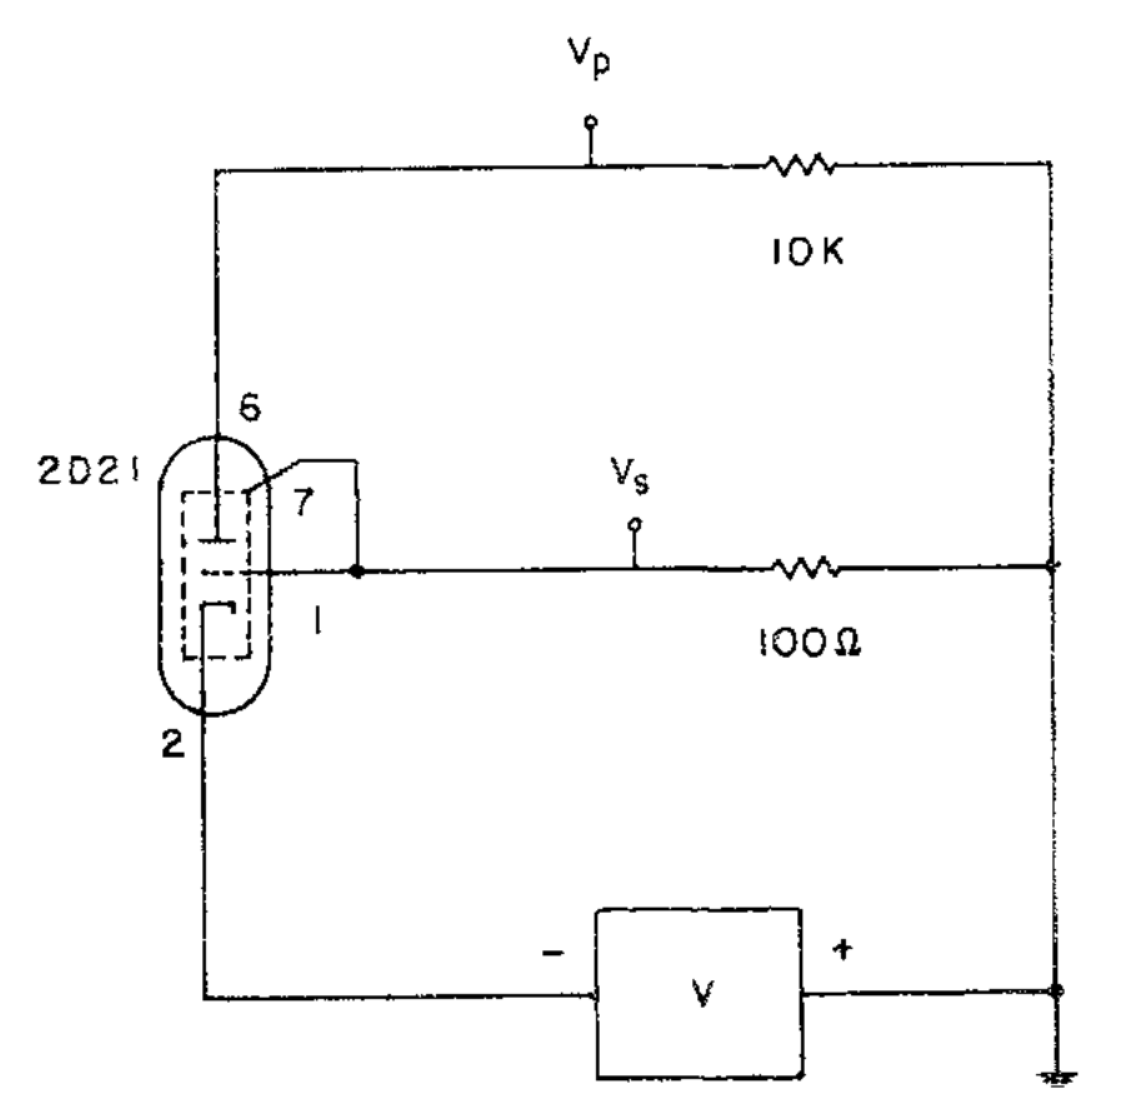
\includegraphics[width=.95\linewidth]{ramsauer_exp.png}
  \caption{Circuit diagram of the experimental setup.}
  \label{fig:1}
\end{figure}

The experiment was set up as per \autoref{fig:1} with a DC power supply set at a constant 4 V as the heater voltage, connected to the 2D21 thyratron tube containing the xenon gas. Two digital multimeters were used to measure the voltage across the 100 and 10k $\Upomega$ resistors (with 5\% tolerances each), the shield and plate currents, respectively. A separate DC power supplied the accelerating electrons into the filament, varied from 0-12 V at varying intervals.

The shield ($V_s$) and plate ($V_p$) voltages were measured both for the xenon gas at room temperature and when frozen with liquid nitrogen, extra care was taken to not shatter the filament with the cold, which effectively "removed" the scattering medium. With the voltages acquired and the associated resistances known, the shield ($I_s$, $I_s^*$) and plate ($I_p$, $I_p^*$) currents were measured using Ohm's law $I=V/R$ for the xenon at room and frozen temperatures, respectively.

With this data, the probability of scattering was acquired by applying Ohm's law to \autoref{eq:1} to obtain the following relation for easier calculation \cite{uwmadison_ramsauer}:

\begin{equation}
  P=1-\frac{V_p V_s^*}{V_s V_p^*}
\end{equation}

The probability of scattering was then be plotted against the electron momentum, which is proportional to the square root of the voltage $\sqrt{V_{accel} - V_s}$, demonstrating the Ramsauer-Townsend Effect.

Corrections for the mean emission ($\bar{V}$) and contact ($V_c$) potentials were found by reversing the polarity for the frozen xenon gas and then applying the corrections to the electron momentum $\sqrt{V - V_s + V_c + \bar{V}}$. To obtain these values, a plot of the natural logarithm of this inverse current was taken against the voltage. The contact potential $\bar{V}$ was obtained from the linear fit of this data, and the contact potential $V_c$ was taken as the "knee" of the same data when categorised and split into saturated and retarding regions and fit linearly. 

\section{Results} \label{sec:4}

Values for the Ramsauer-Townsend effect were obtained and shown graphically for the full 1-12 V range for the xenon gas both at room temperature and when frozen with liquid nitrogen, shown in \autoref{fig:A1}, and zoomed in for the 1-5 V range in \autoref{fig:2}. For this, the plate current $I_p$ was plotted against the accelerating electron voltage $V_{accel}$.

\begin{figure}[H]
  \centering
  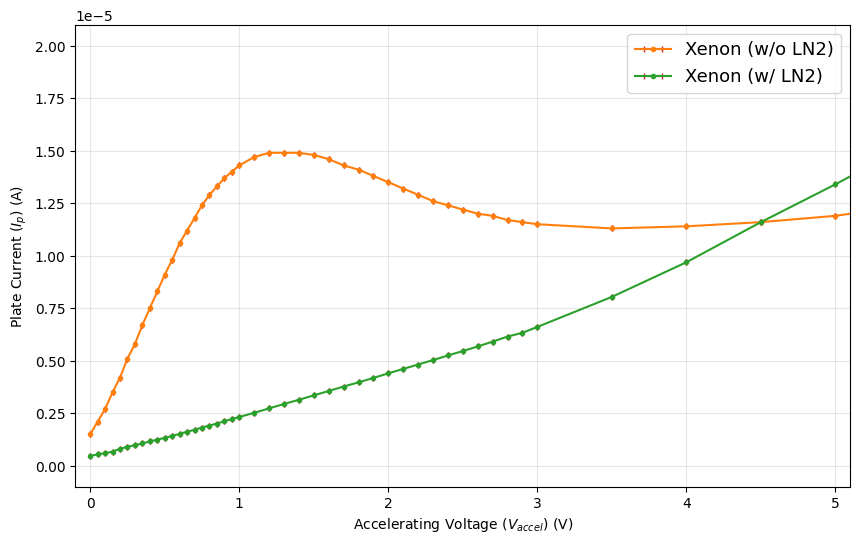
\includegraphics[width=.94\linewidth]{ramsauer_up5.png}
  \caption{Ramsauer-Townsend effect for the xenon gas at room temperature and frozen with LN2.}
  \label{fig:2}
\end{figure}

\begin{figure}[b]
  \centering
  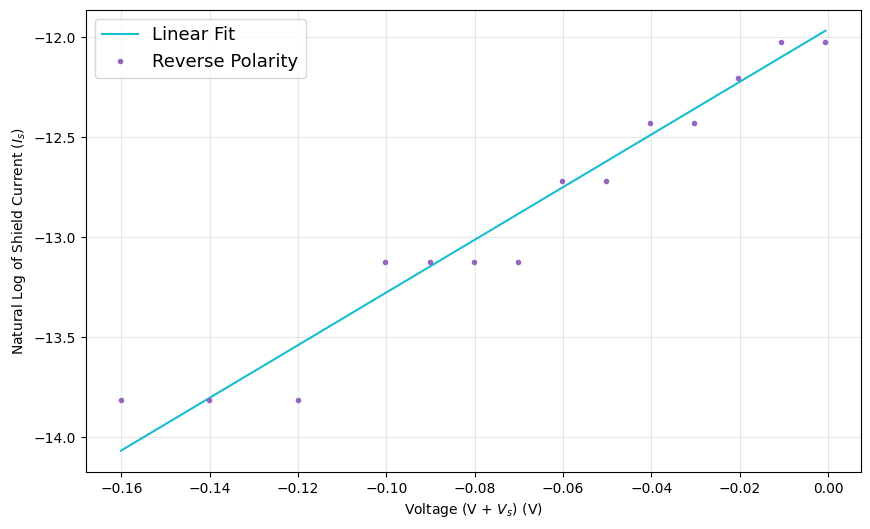
\includegraphics[width=.94\linewidth]{RT_revpollin.png}
  \caption{Ramsauer-Townsend effect in reverse polarity for frozen xenon with LN2 and fitted linearly.}
  \label{fig:3}
\end{figure}

With the polarity of the circuit reversed, values were taken again for the xenon gas frozen with the liquid nitrogen. The natural logarithm of the shield current $\ln(I_s)$ against the voltage ($V+V_s$) was plotted with a linear fit to the values, shown in \autoref{fig:3}. With the slope of this linear fit ($m=13.16 \pm 5.19$), a value for the mean emission potential $\bar{V}$ was calculated using the relationship $\lvert m \rvert = 3/2\bar{V}$. The resulting mean emission potential was found to be $\bar{V}=0.11\pm 0.045$ V.

\begin{figure}[H]
  \centering
  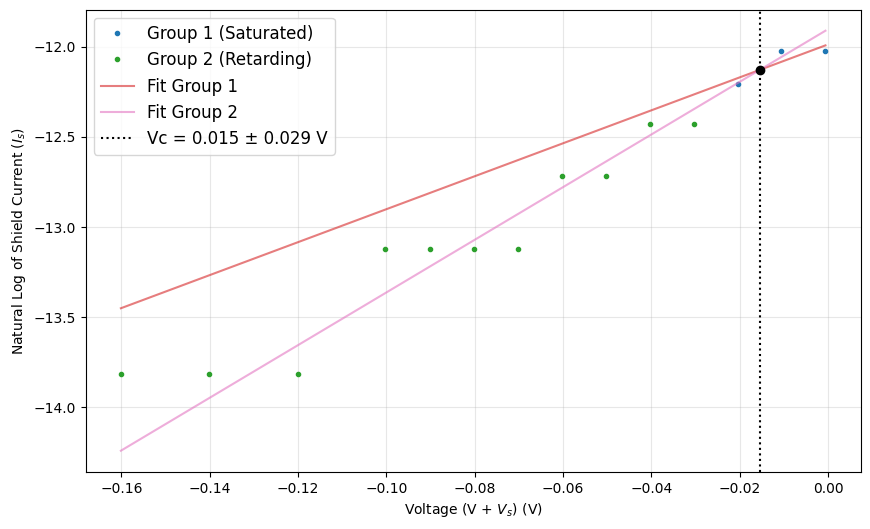
\includegraphics[width=.94\linewidth]{RT_Vc.png}
  \caption{Ramsauer-Townsend effect in reverse polarity for frozen xenon with LN2 and fitted with twice linearly for a saturated and retarding region and a 'knee' at the intersection.}
  \label{fig:4}
\end{figure}

With the same inverse polarity dataset for the frozen xenon gas, the data was split visually into a saturation (blue) and retarding (green) group with two separate and respective linear fits, shown in \autoref{fig:4}. The point at which these lines intersected was regarded as the 'knee' corresponding to the value of the contact potential $V_c$, found to be $V_c = 0.0155 \pm 0.0285$ V. As this value was calculated using the intersection of two lines, the following error propagation formula was used \cite{stackexchange_uncertainty_intersection}:

\vspace{-2ex}
\begin{equation*}
  \Delta x = x \sqrt{\frac{(\Delta c_2)^2 + (\Delta c_1)^2}{(c_2 - c_1)^2} + \frac{(\Delta m_1)^2 + (\Delta m_2)^2}{(m_1 - m_2)^2}}
\end{equation*}

\begin{figure}[hb]
  \centering
  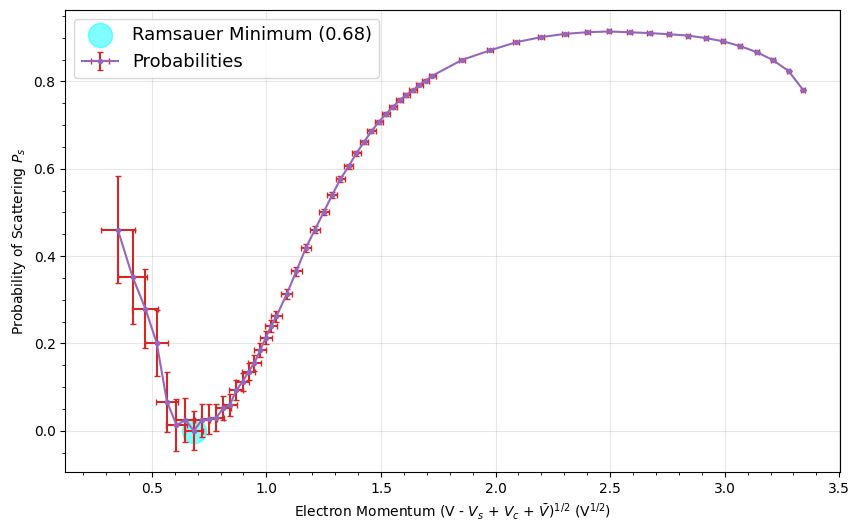
\includegraphics[width=.94\linewidth]{RTprob_correct.png}
  \caption{Probability of scattering corrected with the mean thermal emission and contact potentials.}
  \label{fig:5}
\end{figure}

The probability of scattering $P_s$ was plotted against the square root of the total voltage corrected for the obtained mean emission ($\bar{V}$) and contact potentials ($V_c$) to become (V - $V_s + V_c + \bar{V}$)$^{1/2}$, the corrected electron momentum, shown in \autoref{fig:5}. The uncorrected plot for the probability of scattering is shown in \autoref{fig:A2}. The Ramsauer minimum was found to be a scattering probability of $P_{s,\text{min}}=0.0004 \pm 0.0447$ at an electron momentum of $\sqrt{V}_{\text{min}}=0.6829 \pm 0.0390\; \text{V}^{1/2}$.

\section{Analysis and Discussion} \label{sec:5}

This experiment clearly demonstrated the expected non-classical behaviour of electrons scattering off of the xenon noble gas for low accelerating voltages, the Ramsauer-Townsend effect. Classically, the atoms would be modelled as hard spheres with a constant scattering cross-section, however the data shows a distinct minimum in the scattering probability $P_s$ as electron momentum increases.

This effect is observed in \autoref{fig:5}, in which the corrected scattering probability has a sharp drop that reaches a minimum of $P_{s,\text{min}}=0.0004 \pm 0.0447$ at an electron momentum of $\sqrt{V}_{\text{min}}=0.6829 \pm 0.0390\; \text{V}^{1/2}$. This minimum corresponds to the point at which the xenon gas atoms become effectively "transparent" to the incident electrons, consistent with the quantum-mechanical model of the phase shift of the $l=0$ (s-waves) partial waves at $\delta_0=\pi$ discussed in the introductory theory, in which scattering contribution of the s-waves vanishes.

By reversing the polarity for the frozen xenon gas and preforming two different linear fittings, the mean emission $\bar{V}$ and contact potentials $V_c$ were found and applied as corrections for the probability of scattering plot to align with theoretical expectations. These values were determined as: $\bar{V}=0.11\pm 0.045 \; \text{V}$ and $V_c = 0.0155 \pm 0.0285\; \text{V}$. 

The mean emission potential is within reasonable agreement of the expected value calculated by Woolsey \cite{woolsey1971extension} of $\bar{V} = 0.15 \pm 0.03 \;\text{V}$, with slight discrepancies likely attributed to possible fluctuations in the heater voltage DC supply or the 5\% tolerances of the resistors used. Additionally, if the filament was unevenly heated or cooled it may have led to complications in the natural logarithm of the shield currents ($I_s$) calculations for \autoref{fig:3}.

The contact potential, however, showed a very significant deviation from the expected value calculated by Woolsey \cite{woolsey1971extension} of $V_c = 0.2 \pm 0.04 \;\text{V}$. This discrepancy can be confidently attributed to the identification of the "knee" in \autoref{fig:4} and the near identical slopes for both the saturated and retarding regions. This can be seen in \autoref{fig:A3}, in which by dividing the data in a specific way that does not necessarily agree with the visual "knee", a value of $V_c = 0.21 \pm 0.5202 \;\text{V}$ is obtained, agreeing with the theoretically expected value. Thus, it can be confirmed that the greatest source of systematic error is indeed the selection of data points in each subgroup. Furthermore, data obtained for these extremely low voltages is often more susceptible to electronic noise and the 5\% tolerance in both resistors which propagates through the calculations for current. Additionally, only values for incredibly low voltages were able to be obtained, but if a more sensitive multimeter had been present, then likely a greater range of data could have been obtained.

The accuracy of the scattering probabilities $P_s$ were also highly dependent on the efficiency of the xenon freezing process. If any of the gas had failed to freeze, the desired vacuum-like environment that's created with the liquid nitrogen freezing would be inefficient and undesired scattering may have been present which would influence the $I_s^*$ and $I_p^*$ measurements, resulting in an underestimation of the scattering probability. Despite these likely sources of errors and discrepancies, the shape of the plot was as expected, showcasing the wave-like nature of the electrons that's dominant in low-energy noble gas scattering. The corrections from the mean emission and contact potentials were also vital in shifting the plot and in determining the correct scattering minimum.

\section{Conclusion}

This experiment successfully demonstrated the Ramsauer-Townsend effect and provided a clear demonstration of the wave-particle duality of electrons through their interactions with a noble gas, such as xenon. The observation of a sharp minimum in scattering probability directly contradicts classical expectations of a constant scattering cross-section in the hard spherical atoms model, instead supporting the quantum-mechanical model where the phase shift of the $l=0$ partial waves reaches $\delta_0=\pi$.

The inclusion of the corrections for the mean emission and contact potentials ensured accuracy of the probability quantitative results. The obtained mean emission potential $\bar{V}=0.11\pm 0.045 \; \text{V}$ agreed with the theoretical expectations. Although the obtained result for the contact potential $V_c = 0.0155 \pm 0.0285\; \text{V}$ differed from the expected theoretical values, this experiment highlighted a big discrepancy in the calculation of this value in such that it is incredibly sensitive to the subjective classification and splitting of the data into saturated and retarding groups. The fact that the same data with different group splits could yield a value within expected data $V_c = 0.21 \pm 0.5202 \;\text{V}$ suggests that perhaps a more standardised and constant method or algorithm of identifying the "knee" in reverse polarity plots would ensure better accuracy in values.

Despite any discrepancies in values, this experiment successfully displayed the expected curve of the scattering probabilities plot with a distinct minimum at which the xenon atoms would become essentially "transparent" to the incident electrons, thus verifying the Ramsauer-Townsend phenomenon.

%%%%%%%%%%%%%%%%%%%%

% References - switch to single column
\onecolumn

\bibliographystyle{IEEEtran}
\bibliography{PHYC30170References} \label{sec:ref}

\newpage

% Appendix - single column
\section*{Appendix} \label{sec:A}
\addcontentsline{toc}{section}{Appendix}

\subsection*{Figures}
\addcontentsline{toc}{subsection}{Figures}

\begin{figure}[H]
  \centering
  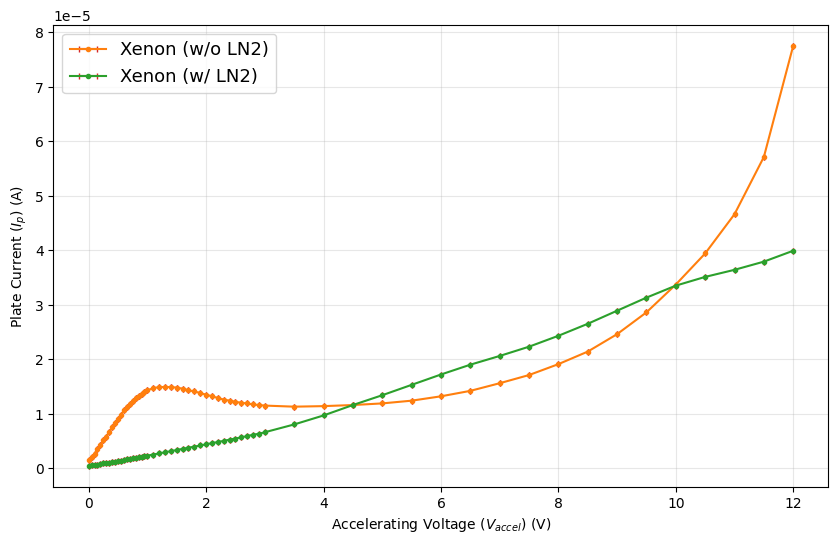
\includegraphics[width=.85\textwidth]{ramsauer_all.png}
  \caption{Ramsauer-Townsend effect for the xenon gas at room temperature and frozen with LN2 for the full range of accelerating voltages observed.}
  \label{fig:A1}
\end{figure}

\begin{figure}[H]
  \centering
  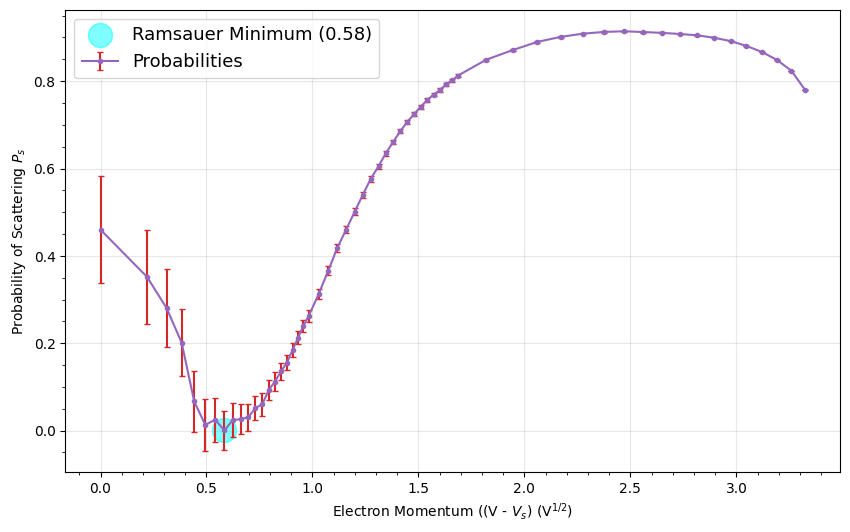
\includegraphics[width=.85\textwidth]{RTprob_uncorrect.png}
  \caption{Probability of scattering uncorrected.}
  \label{fig:A2}
\end{figure}

\begin{figure}[H]
  \centering
  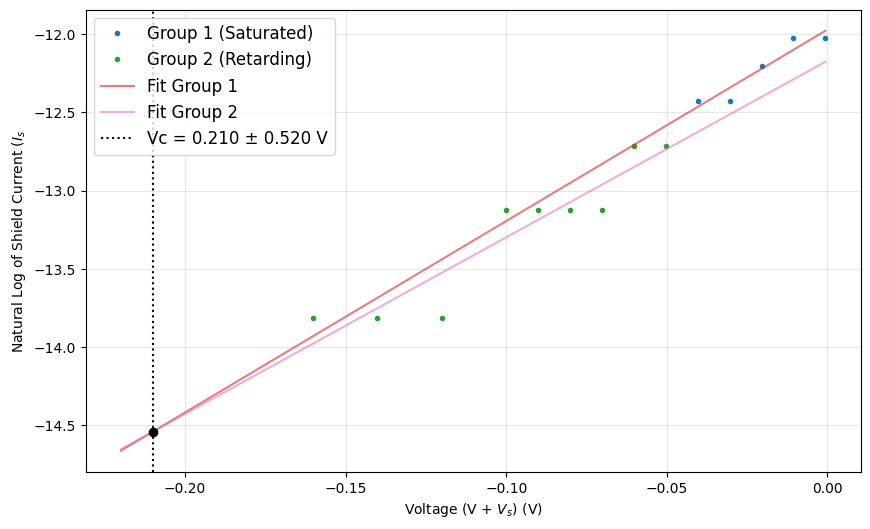
\includegraphics[width=.85\linewidth]{RT_agreeVc.png} 
  \caption{Reverse polarity with data grouped to give an agreeing value to theoretical expectations.}
  \label{fig:A3}
\end{figure}

\subsection*{Tables}
\addcontentsline{toc}{subsection}{Tables}

\begin{longtable}[c]{|
>{\columncolor[HTML]{EFEFEF}}c |c|c|c|c|}
\caption{Table of the raw data for the xenon gas at room temperature.}
\label{tab:1}\\
\hline
Accel. voltage (V) & \cellcolor[HTML]{EFEFEF}(Plate) Vp (V) & \cellcolor[HTML]{EFEFEF}(Shield) Vs (V) & \cellcolor[HTML]{EFEFEF}(Plate) Ip (A) & \cellcolor[HTML]{EFEFEF}(Shield) Is (A) \\ \hline
\endfirsthead
%
\multicolumn{5}{c}%
{{\bfseries Table \thetable\ continued from previous page}} \\
\endhead
%
0                  & 1.50E-03                       & 1.30E-03                       & 1.50E-07                   & 1.30E-05                   \\ \hline
0.05               & 2.10E-03                       & 1.80E-03                       & 2.10E-07                   & 1.80E-05                   \\ \hline
0.1                & 2.70E-03                       & 2.50E-03                       & 2.70E-07                   & 2.50E-05                   \\ \hline
0.15               & 3.50E-03                       & 3.40E-03                       & 3.50E-07                   & 3.40E-05                   \\ \hline
0.2                & 4.20E-03                       & 4.50E-03                       & 4.20E-07                   & 4.50E-05                   \\ \hline
0.25               & 5.10E-03                       & 5.80E-03                       & 5.10E-07                   & 5.80E-05                   \\ \hline
0.3                & 5.80E-03                       & 7.10E-03                       & 5.80E-07                   & 7.10E-05                   \\ \hline
0.35               & 6.70E-03                       & 8.60E-03                       & 6.70E-07                   & 8.60E-05                   \\ \hline
0.4                & 7.50E-03                       & 1.04E-02                       & 7.50E-07                   & 1.04E-04                   \\ \hline
0.45               & 8.30E-03                       & 1.21E-02                       & 8.30E-07                   & 1.21E-04                   \\ \hline
0.5                & 9.10E-03                       & 1.39E-02                       & 9.10E-07                   & 1.39E-04                   \\ \hline
0.55               & 9.80E-03                       & 1.58E-02                       & 9.80E-07                   & 1.58E-04                   \\ \hline
0.6                & 1.06E-02                       & 1.78E-02                       & 1.06E-06                   & 1.78E-04                   \\ \hline
0.65               & 1.12E-02                       & 1.99E-02                       & 1.12E-06                   & 1.99E-04                   \\ \hline
0.7                & 1.18E-02                       & 2.20E-02                       & 1.18E-06                   & 2.20E-04                   \\ \hline
0.75               & 1.24E-02                       & 2.42E-02                       & 1.24E-06                   & 2.42E-04                   \\ \hline
0.8                & 1.29E-02                       & 2.64E-02                       & 1.29E-06                   & 2.64E-04                   \\ \hline
0.85               & 1.33E-02                       & 2.88E-02                       & 1.33E-06                   & 2.88E-04                   \\ \hline
0.9                & 1.37E-02                       & 3.12E-02                       & 1.37E-06                   & 3.12E-04                   \\ \hline
0.95               & 1.40E-02                       & 3.36E-02                       & 1.40E-06                   & 3.36E-04                   \\ \hline
1                  & 1.43E-02                       & 3.60E-02                       & 1.43E-06                   & 3.60E-04                   \\ \hline
1.1                & 1.47E-02                       & 4.09E-02                       & 1.47E-06                   & 4.09E-04                   \\ \hline
1.2                & 1.49E-02                       & 4.62E-02                       & 1.49E-06                   & 4.62E-04                   \\ \hline
1.3                & 1.49E-02                       & 5.16E-02                       & 1.49E-06                   & 5.16E-04                   \\ \hline
1.4                & 1.49E-02                       & 5.68E-02                       & 1.49E-06                   & 5.68E-04                   \\ \hline
1.5                & 1.48E-02                       & 6.24E-02                       & 1.48E-06                   & 6.24E-04                   \\ \hline
1.6                & 1.46E-02                       & 6.82E-02                       & 1.46E-06                   & 6.82E-04                   \\ \hline
1.7                & 1.43E-02                       & 7.39E-02                       & 1.43E-06                   & 7.39E-04                   \\ \hline
1.8                & 1.41E-02                       & 7.98E-02                       & 1.41E-06                   & 7.98E-04                   \\ \hline
1.9                & 1.38E-02                       & 8.60E-02                       & 1.38E-06                   & 8.60E-04                   \\ \hline
2                  & 1.35E-02                       & 9.23E-02                       & 1.35E-06                   & 9.23E-04                   \\ \hline
2.1                & 1.32E-02                       & 9.84E-02                       & 1.32E-06                   & 9.84E-04                   \\ \hline
2.2                & 1.29E-02                       & 1.05E-01                       & 1.29E-06                   & 1.05E-03                   \\ \hline
2.3                & 1.26E-02                       & 1.11E-01                       & 1.26E-06                   & 1.11E-03                   \\ \hline
2.4                & 1.24E-02                       & 1.17E-01                       & 1.24E-06                   & 1.17E-03                   \\ \hline
2.5                & 1.22E-02                       & 1.24E-01                       & 1.22E-06                   & 1.24E-03                   \\ \hline
2.6                & 1.20E-02                       & 1.30E-01                       & 1.20E-06                   & 1.30E-03                   \\ \hline
2.7                & 1.19E-02                       & 1.36E-01                       & 1.19E-06                   & 1.36E-03                   \\ \hline
2.8                & 1.17E-02                       & 1.43E-01                       & 1.17E-06                   & 1.43E-03                   \\ \hline
2.9                & 1.16E-02                       & 1.49E-01                       & 1.16E-06                   & 1.49E-03                   \\ \hline
3                  & 1.15E-02                       & 1.56E-01                       & 1.15E-06                   & 1.56E-03                   \\ \hline
3.5                & 1.13E-02                       & 1.89E-01                       & 1.13E-06                   & 1.89E-03                   \\ \hline
4                  & 1.14E-02                       & 0.219                          & 1.14E-06                   & 0.00219                    \\ \hline
4.5                & 1.16E-02                       & 0.254                          & 1.16E-06                   & 0.00254                    \\ \hline
5                  & 1.19E-02                       & 0.288                          & 1.19E-06                   & 0.00288                    \\ \hline
5.5                & 1.24E-02                       & 0.323                          & 1.24E-06                   & 0.00323                    \\ \hline
6                  & 1.32E-02                       & 0.36                           & 1.32E-06                   & 0.0036                     \\ \hline
6.5                & 1.42E-02                       & 0.399                          & 1.42E-06                   & 0.00399                    \\ \hline
7                  & 1.56E-02                       & 0.439                          & 1.56E-06                   & 0.00439                    \\ \hline
7.5                & 1.71E-02                       & 0.48                           & 1.71E-06                   & 0.0048                     \\ \hline
8                  & 1.91E-02                       & 0.524                          & 1.91E-06                   & 0.00524                    \\ \hline
8.5                & 2.14E-02                       & 0.568                          & 2.14E-06                   & 0.00568                    \\ \hline
9                  & 2.46E-02                       & 0.616                          & 2.46E-06                   & 0.00616                    \\ \hline
9.5                & 2.86E-02                       & 0.663                          & 2.86E-06                   & 0.00663                    \\ \hline
10                 & 3.37E-02                       & 0.712                          & 3.37E-06                   & 0.00712                    \\ \hline
10.5               & 3.94E-02                       & 0.763                          & 3.94E-06                   & 0.00763                    \\ \hline
11                 & 4.66E-02                       & 0.815                          & 4.66E-06                   & 0.00815                    \\ \hline
11.5               & 5.71E-02                       & 0.873                          & 5.71E-06                   & 0.00873                    \\ \hline
12                 & 7.75E-02                       & 0.951                          & 7.75E-06                   & 0.00951                    \\ \hline
\end{longtable}

\begin{longtable}[c]{|
>{\columncolor[HTML]{EFEFEF}}c |c|c|c|c|}
\caption{Table of the raw data for the xenon gas frozen with liquid nitrogen.}
\label{tab:2}\\
\hline
Accel. voltage (V) & \cellcolor[HTML]{EFEFEF}(Plate) Vp (V) & \cellcolor[HTML]{EFEFEF}(Shield) Vs (V) & \cellcolor[HTML]{EFEFEF}(Plate) Ip (A) & \cellcolor[HTML]{EFEFEF}(Shield) Is (A) \\ \hline
\endfirsthead
%
\multicolumn{5}{c}%
{{\bfseries Table \thetable\ continued from previous page}} \\
\endhead
%
0                  & 4.70E-03                               & 2.20E-03                                & 4.70E-07                               & 2.20E-05                                \\ \hline
0.05               & 5.40E-03                               & 3.00E-03                                & 5.40E-07                               & 3.00E-05                                \\ \hline
0.1                & 6.00E-03                               & 4.00E-03                                & 6.00E-07                               & 4.00E-05                                \\ \hline
0.15               & 6.70E-03                               & 5.20E-03                                & 6.70E-07                               & 5.20E-05                                \\ \hline
0.2                & 8.10E-03                               & 8.10E-03                                & 8.10E-07                               & 8.10E-05                                \\ \hline
0.25               & 9.00E-03                               & 1.01E-02                                & 9.00E-07                               & 1.01E-04                                \\ \hline
0.3                & 9.80E-03                               & 1.17E-02                                & 9.80E-07                               & 1.17E-04                                \\ \hline
0.35               & 1.06E-02                               & 1.36E-02                                & 1.06E-06                               & 1.36E-04                                \\ \hline
0.4                & 1.16E-02                               & 1.57E-02                                & 1.16E-06                               & 1.57E-04                                \\ \hline
0.45               & 1.24E-02                               & 1.76E-02                                & 1.24E-06                               & 1.76E-04                                \\ \hline
0.5                & 1.33E-02                               & 1.97E-02                                & 1.33E-06                               & 1.97E-04                                \\ \hline
0.55               & 1.42E-02                               & 2.17E-02                                & 1.42E-06                               & 2.17E-04                                \\ \hline
0.6                & 1.52E-02                               & 2.40E-02                                & 1.52E-06                               & 2.40E-04                                \\ \hline
0.65               & 1.62E-02                               & 2.61E-02                                & 1.62E-06                               & 2.61E-04                                \\ \hline
0.7                & 1.71E-02                               & 2.83E-02                                & 1.71E-06                               & 2.83E-04                                \\ \hline
0.75               & 1.82E-02                               & 3.07E-02                                & 1.82E-06                               & 3.07E-04                                \\ \hline
0.8                & 1.91E-02                               & 3.30E-02                                & 1.91E-06                               & 3.30E-04                                \\ \hline
0.85               & 2.01E-02                               & 3.55E-02                                & 2.01E-06                               & 3.55E-04                                \\ \hline
0.9                & 2.12E-02                               & 3.80E-02                                & 2.12E-06                               & 3.80E-04                                \\ \hline
0.95               & 2.22E-02                               & 4.05E-02                                & 2.22E-06                               & 4.05E-04                                \\ \hline
1                  & 2.32E-02                               & 4.31E-02                                & 2.32E-06                               & 4.31E-04                                \\ \hline
1.1                & 2.52E-02                               & 4.82E-02                                & 2.52E-06                               & 4.82E-04                                \\ \hline
1.2                & 2.73E-02                               & 5.37E-02                                & 2.73E-06                               & 5.37E-04                                \\ \hline
1.3                & 2.94E-02                               & 5.92E-02                                & 2.94E-06                               & 5.92E-04                                \\ \hline
1.4                & 3.14E-02                               & 6.46E-02                                & 3.14E-06                               & 6.46E-04                                \\ \hline
1.5                & 3.35E-02                               & 7.05E-02                                & 3.35E-06                               & 7.05E-04                                \\ \hline
1.6                & 3.56E-02                               & 7.65E-02                                & 3.56E-06                               & 7.65E-04                                \\ \hline
1.7                & 3.77E-02                               & 8.25E-02                                & 3.77E-06                               & 8.25E-04                                \\ \hline
1.8                & 3.97E-02                               & 8.87E-02                                & 3.97E-06                               & 8.87E-04                                \\ \hline
1.9                & 4.18E-02                               & 9.50E-02                                & 4.18E-06                               & 9.50E-04                                \\ \hline
2                  & 4.40E-02                               & 1.02E-01                                & 4.40E-06                               & 1.02E-03                                \\ \hline
2.1                & 4.61E-02                               & 1.08E-01                                & 4.61E-06                               & 1.08E-03                                \\ \hline
2.2                & 4.82E-02                               & 1.15E-01                                & 4.82E-06                               & 1.15E-03                                \\ \hline
2.3                & 5.03E-02                               & 1.22E-01                                & 5.03E-06                               & 1.22E-03                                \\ \hline
2.4                & 5.25E-02                               & 1.28E-01                                & 5.25E-06                               & 1.28E-03                                \\ \hline
2.5                & 5.46E-02                               & 1.35E-01                                & 5.46E-06                               & 1.35E-03                                \\ \hline
2.6                & 5.68E-02                               & 1.42E-01                                & 5.68E-06                               & 1.42E-03                                \\ \hline
2.7                & 5.91E-02                               & 1.49E-01                                & 5.91E-06                               & 1.49E-03                                \\ \hline
2.8                & 6.15E-02                               & 1.56E-01                                & 6.15E-06                               & 1.56E-03                                \\ \hline
2.9                & 6.33E-02                               & 1.61E-01                                & 6.33E-06                               & 1.61E-03                                \\ \hline
3                  & 6.61E-02                               & 1.68E-01                                & 6.61E-06                               & 1.68E-03                                \\ \hline
3.5                & 8.04E-02                               & 2.03E-01                                & 8.04E-06                               & 2.03E-03                                \\ \hline
4                  & 9.69E-02                               & 0.24                                    & 9.69E-06                               & 0.0024                                  \\ \hline
4.5                & 1.16E-01                               & 0.28                                    & 1.16E-05                               & 0.0028                                  \\ \hline
5                  & 1.34E-01                               & 0.32                                    & 1.34E-05                               & 0.0032                                  \\ \hline
5.5                & 1.53E-01                               & 0.364                                   & 1.53E-05                               & 0.00364                                 \\ \hline
6                  & 1.72E-01                               & 0.41                                    & 1.72E-05                               & 0.0041                                  \\ \hline
6.5                & 1.90E-01                               & 0.458                                   & 1.90E-05                               & 0.00458                                 \\ \hline
7                  & 0.206                                  & 0.508                                   & 0.0000206                              & 0.00508                                 \\ \hline
7.5                & 0.223                                  & 0.56                                    & 0.0000223                              & 0.0056                                  \\ \hline
8                  & 0.243                                  & 0.614                                   & 0.0000243                              & 0.00614                                 \\ \hline
8.5                & 0.265                                  & 0.669                                   & 0.0000265                              & 0.00669                                 \\ \hline
9                  & 0.289                                  & 0.729                                   & 0.0000289                              & 0.00729                                 \\ \hline
9.5                & 0.313                                  & 0.786                                   & 0.0000313                              & 0.00786                                 \\ \hline
10                 & 0.335                                  & 0.845                                   & 0.0000335                              & 0.00845                                 \\ \hline
10.5               & 0.351                                  & 0.905                                   & 0.0000351                              & 0.00905                                 \\ \hline
11                 & 0.364                                  & 0.964                                   & 0.0000364                              & 0.00964                                 \\ \hline
11.5               & 0.379                                  & 1.022                                   & 0.0000379                              & 0.01022                                 \\ \hline
12                 & 0.399                                  & 1.077                                   & 0.0000399                              & 0.01077                                 \\ \hline
\end{longtable}

% Please add the following required packages to your document preamble:
% \usepackage[table,xcdraw]{xcolor}
% Beamer presentation requires \usepackage{colortbl} instead of \usepackage[table,xcdraw]{xcolor}
% \usepackage{longtable}
% Note: It may be necessary to compile the document several times to get a multi-page table to line up properly
\begin{longtable}[c]{|
>{\columncolor[HTML]{EFEFEF}}c |c|c|c|c|}
\caption{Table of the raw data for the xenon gas frozen with liquid nitrogen with reversed polarity.}
\label{tab:3}\\
\hline
Accel. voltage (V) & \cellcolor[HTML]{EFEFEF}(Plate) Vp (V) & \cellcolor[HTML]{EFEFEF}(Shield) Vs (V) & \cellcolor[HTML]{EFEFEF}(Plate) Ip (A) & \cellcolor[HTML]{EFEFEF}(Shield) Is (A) \\ \hline
\endfirsthead
%
\multicolumn{5}{c}%
{{\bfseries Table \thetable\ continued from previous page}} \\
\endhead
%
0                  & 1.90E-03                               & 6.00E-04                                & 1.90E-07                               & 6.00E-06                                \\ \hline
0.01               & 1.80E-03                               & 6.00E-04                                & 1.80E-07                               & 6.00E-06                                \\ \hline
0.02               & 1.60E-03                               & 5.00E-04                                & 1.60E-07                               & 5.00E-06                                \\ \hline
0.03               & 1.50E-03                               & 4.00E-04                                & 1.50E-07                               & 4.00E-06                                \\ \hline
0.04               & 1.30E-03                               & 4.00E-04                                & 1.30E-07                               & 4.00E-06                                \\ \hline
0.05               & 1.20E-03                               & 3.00E-04                                & 1.20E-07                               & 3.00E-06                                \\ \hline
0.06               & 1.00E-03                               & 3.00E-04                                & 1.00E-07                               & 3.00E-06                                \\ \hline
0.07               & 9.00E-04                               & 2.00E-04                                & 9.00E-08                               & 2.00E-06                                \\ \hline
0.08               & 8.00E-04                               & 2.00E-04                                & 8.00E-08                               & 2.00E-06                                \\ \hline
0.09               & 7.00E-04                               & 2.00E-04                                & 7.00E-08                               & 2.00E-06                                \\ \hline
0.1                & 7.00E-04                               & 2.00E-04                                & 7.00E-08                               & 2.00E-06                                \\ \hline
0.12               & 6.00E-04                               & 1.00E-04                                & 6.00E-08                               & 1.00E-06                                \\ \hline
0.14               & 4.00E-04                               & 1.00E-04                                & 4.00E-08                               & 1.00E-06                                \\ \hline
0.16               & 3.00E-04                               & 1.00E-04                                & 3.00E-08                               & 1.00E-06                                \\ \hline
0.18               & 3.00E-04                               & 0.00E+00                                & 3.00E-08                               & 0.00E+00                                \\ \hline
0.2                & 2.00E-04                               & 0.00E+00                                & 2.00E-08                               & 0.00E+00                                \\ \hline
0.25               & 1.00E-04                               & 0.00E+00                                & 1.00E-08                               & 0.00E+00                                \\ \hline
0.3                & 0.00E+00                               & 0.00E+00                                & 0.00E+00                               & 0.00E+00                                \\ \hline
\end{longtable}

\addcontentsline{toc}{subsection}{Code}

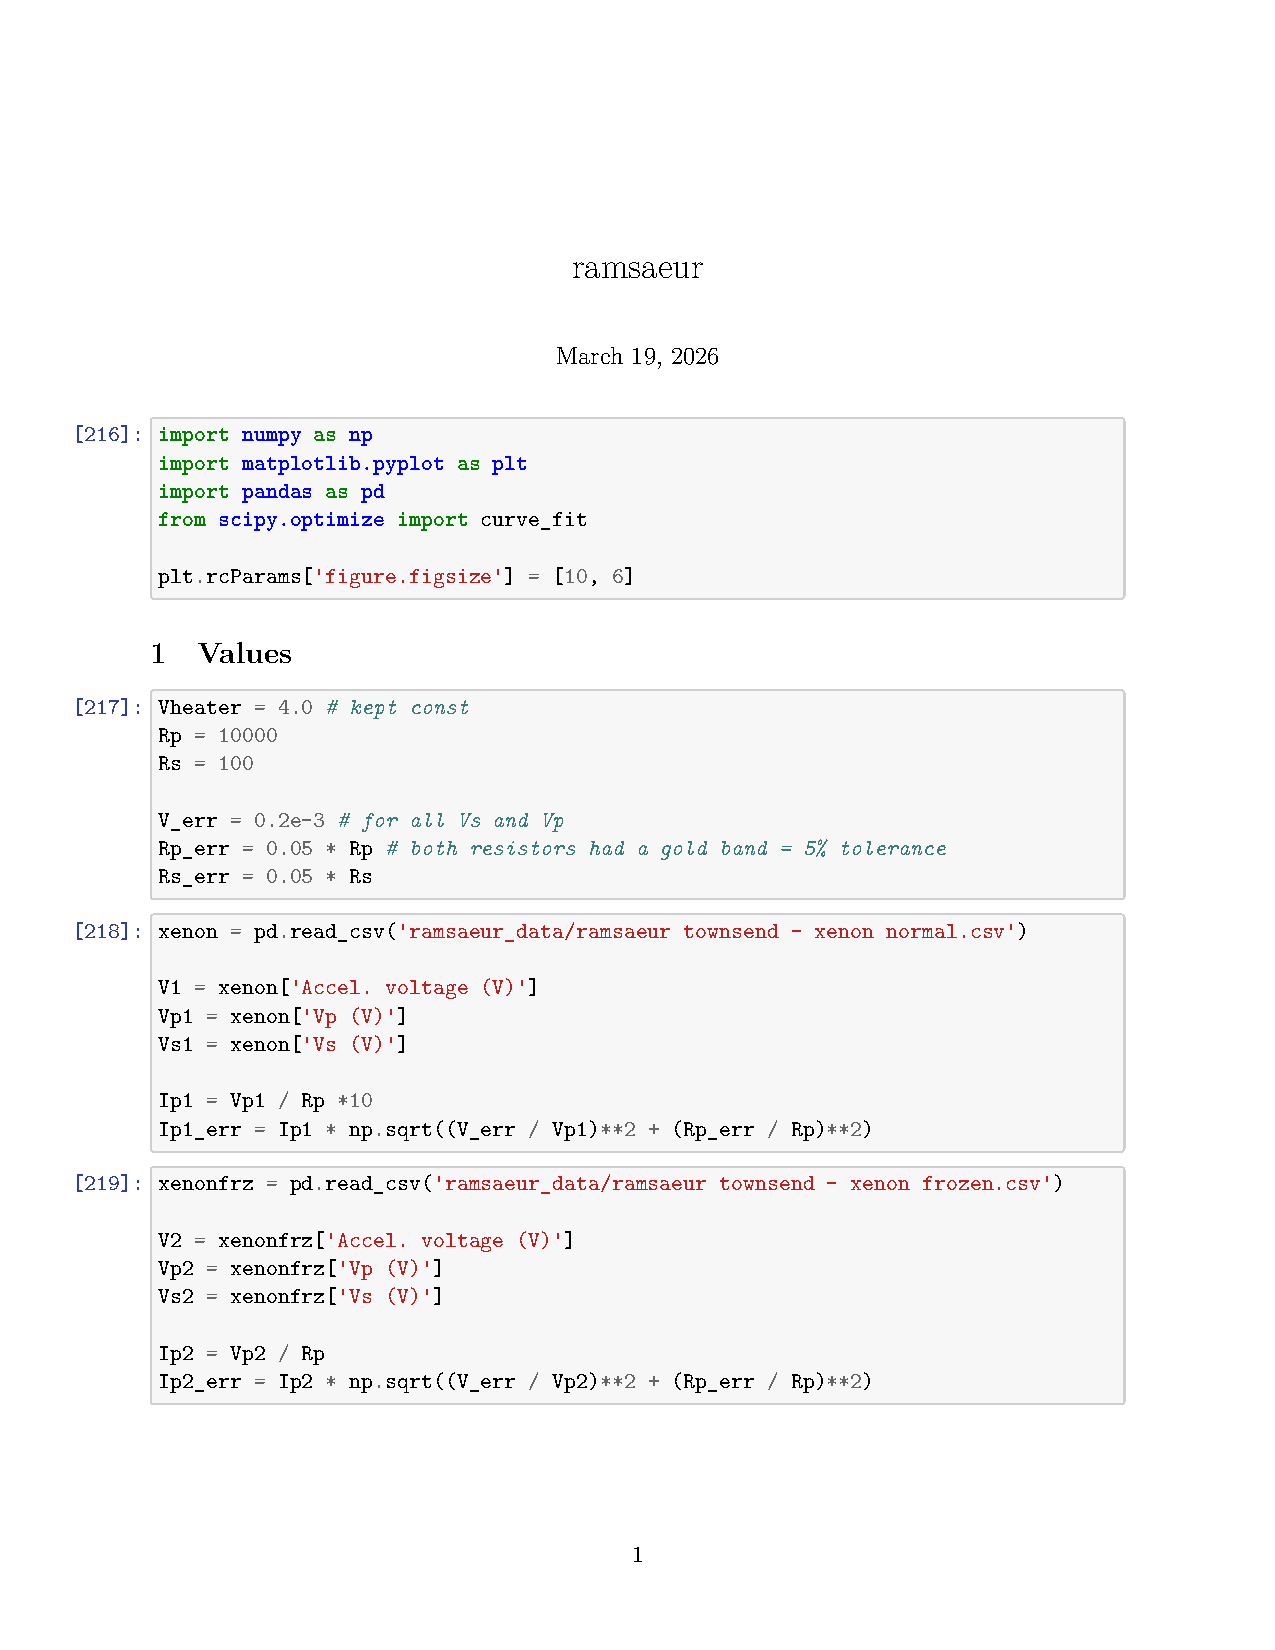
\includepdf[pages={1-8}]{ramsaeur.pdf}

\end{document}